% ============================================================================
\section{Expert Assessment of Procedural Correctness}
\label{sec:expert}

The automatic metric compares a generated reply with one recorded reply. To check
whether that similarity tracks procedural correctness, we asked support engineers
to rate a blinded sample. The sample contains 105 changed pairs, 35 in each of
three arms: familiar procedures with blind feedback, new procedures with blind
feedback, and new procedures with conditioned feedback. A pair is eligible only if
the feedback answer differs from the baseline answer; unchanged pairs would add no
information. The sample is stratified by resolving team, A/B order is randomized
and balanced within each arm, and no ticket appears in two arms. The study is a
validity check, not a confirmatory trial: the arms contain only 2--7 discordant
pairs, and one expert has completed the sample while the second is in progress.

For each reply the expert marked correct, partially correct, incorrect or cannot
judge, flagged a wrong or unsafe step and a missing required step, and then chose
the better reply, with equal, both incorrect and cannot judge as explicit options.
Strict correctness counts only ``correct''; lenient correctness also counts
``partially correct''. Intervals are paired bootstrap intervals over tickets;
p-values are exact McNemar tests on discordant pairs. Table~\ref{tab:expert} and
Figure~\ref{fig:expert} report the first expert's results.

\Table[!btp](width=\textwidth){Blinded expert assessment of procedural correctness
(E1; 105 items, 35 per arm). Strict correctness counts only ``correct''. Intervals
are paired bootstrap intervals over tickets; $p$ is the exact McNemar test on
discordant pairs. Four items were cannot-judge and are excluded from the paired
analysis. Discordant pairs: 7, 3 and 2. Across all 105 items: 42 equal, 32 both
incorrect, 2 cannot judge. On the familiar arm the feedback replies are 173
characters longer; the expert preference tracks length (Spearman $+0.63$) and is
zero among length-matched pairs. The second expert is in progress; agreement is not
yet reported.\label{tab:expert}}{
\begin{tabular}{@{}lrrrrr@{}}
\toprule
Arm & $n$ & Baseline & Feedback & $\Delta$ [95\,\% CI] & $p$ \\
\midrule
Familiar, blind       & 34 & 0.647 & 0.794 & $+0.147$ $[0.000, +0.294]$ & .25 \\
Strict, blind         & 33 & 0.545 & 0.515 & $-0.030$ $[-0.121, +0.061]$ & 1.00 \\
Strict, conditioned   & 34 & 0.559 & 0.559 & $0.000$ $[-0.088, +0.088]$ & 1.00 \\
\bottomrule
\end{tabular}}

\begin{figure*}[!t]
\centering
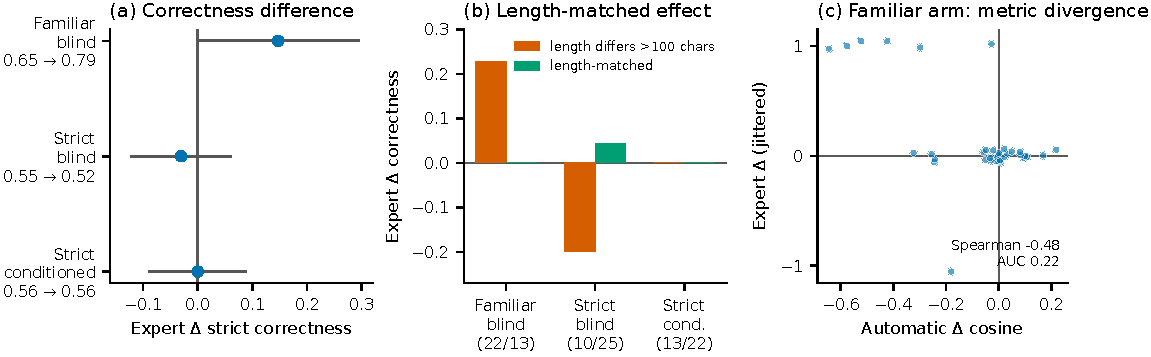
\includegraphics[width=\textwidth]{revision_ieee_access/03_manuscript/figures/fig3_expert_evaluation.pdf}
\caption{Expert assessment (E1). (a)~Strict-correctness difference between feedback
and baseline with 95\,\% paired bootstrap intervals; the labels show the baseline
and feedback rates. (b)~Effect among length-matched pairs versus pairs whose lengths
differ by more than 100 characters; sample sizes are unmatched/matched. (c)~Automatic
cosine difference versus expert difference on the familiar arm; the two measures
point in opposite directions.}
\label{fig:expert}
\end{figure*}

Three results matter. First, on the strict panels the expert does not confirm
benefit or harm: both intervals include zero and the point estimates are within $\pm0.03$,
matching the small automatic effects there. Second, the familiar arm shows a raw
$+0.147$, but the feedback replies are 173 characters longer and the expert
preference tracks that difference (Spearman $+0.63$); among pairs whose lengths
differ by at most 100 characters the effect is exactly zero (n=13). The apparent
benefit on familiar procedures is a preference for longer, more detailed replies,
not a demonstrated procedural improvement. Third, the expert and the cosine metric
point in opposite directions on that arm (expert $+0.147$, automatic $-0.088$;
Spearman $-0.48$, AUC 0.22). Neither measure is a clean criterion: cosine rewards
similarity to one recorded reply, and the expert is sensitive to answer length.

The preference data show why the per-reply correctness rating was necessary.
Across the sample, 42 items were rated equal and 32 both incorrect; a raw A/B
preference alone would have hidden a third of the sample as ``both wrong''. The
unsafe-step and missing-step flags were rare (5.7--8.6\,\% for unsafe steps,
0--2.9\,\% for missing steps), so we report them descriptively and do not treat
them as evidence of a safety difference. With 2--7 discordant pairs per arm, the
study can detect only an almost perfectly consistent advantage; the intervals, not
the p-values, are the result. We do not claim that the expert confirms either the
automatic harm or the automatic benefit.

The second expert will be analysed with the same fixed pipeline. When the sample is
complete we will add percent agreement, Cohen's $\kappa$ with a bootstrap interval,
weighted $\kappa$ for the ordinal correctness rating, PABAK/AC1 as a
prevalence-robust sensitivity, and a combined per-item estimate on the common items.
The analysis supports partial overlap: if the second expert does not finish all 105
items, the agreement and combined estimate use the items both experts rated, and
the coverage is reported explicitly. The sample, answers, A/B assignment and
analysis plan are frozen; no item is added or removed after the first rating.
